\documentclass[11pt]{article}

\usepackage[T1]{fontenc}
\usepackage[utf8]{inputenc}
\usepackage[french]{babel}
\usepackage{amsmath, amssymb, amsthm}
\usepackage{graphicx}
\usepackage{geometry}
\usepackage{enumitem}
\usepackage{hyperref}
\usepackage{mdframed}
\usepackage{mathtools}

\geometry{margin=2.5cm}

% --- Macros utiles ---
\newcommand{\RR}{\mathbb{R}}
\newcommand{\NN}{\mathbb{N}}
\newcommand{\acompleter}{\fbox{À compléter}}

% --- Style des cadres ---
\mdfdefinestyle{coursbox}{
  linewidth=0.8pt,
  linecolor=black,
  backgroundcolor=white,
  roundcorner=0pt,
  innertopmargin=8pt,
  innerbottommargin=8pt,
  innerleftmargin=10pt,
  innerrightmargin=10pt,
  skipabove=10pt,
  skipbelow=10pt
}

% --- Environnements simples ---
\newenvironment{remarque}{\par\smallskip\noindent\textbf{Remarque. \\}\ignorespaces}{\par\smallskip}
\newenvironment{exemple}{\par\smallskip\noindent\textbf{Exemple. \\}\ignorespaces}{\par\smallskip}
\newenvironment{exemples}{\par\smallskip\noindent\textbf{Exemples. \\}\ignorespaces}{\par\smallskip}
\newenvironment{demonstration}{\par\smallskip\noindent\textbf{Démonstration. \\}\ignorespaces}{\par\smallskip}
\newenvironment{historique}{\par\smallskip\noindent\textbf{Historique. \\}\ignorespaces}{\par\smallskip}

% --- Environnements encadrés ---
\newmdenv[style=coursbox]{definition}
\newmdenv[style=coursbox]{propriete}
\newmdenv[style=coursbox]{proprietes}

\begin{document}

\begin{definition}
\begin{center}
    {\Huge\bfseries Trigonométrie - 2/2}
\end{center}
\end{definition}

\begin{historique}
Après Ptolémée, les développements significatifs de la trigonométrie furent réalisés en Inde. L'astronome et mathématicien indien Aryabhata (476--550), dans son ouvrage \emph{Arya-Siddhanta}, définit pour la première fois le sinus à partir de la relation entre la moitié d'un angle et la moitié d'une corde, tout en définissant également le cosinus, le contre-sinus (ou sinus verse) et l'inverse du sinus.

Les travaux indiens furent traduits plus tard et améliorés par les mathématiciens islamiques. Au Xe siècle, le mathématicien perse Muhammad ibn Mūsā al-Khwārizmī produisit des tables des sinus et des tangentes, et apporta aussi sa contribution à la trigonométrie sphérique.

Le traité \emph{Canon doctrinæ triangulorum} (1551) de Georg Joachim Rheticus, un élève de Copernic, fut probablement le premier ouvrage dans lequel les fonctions trigonométriques étaient définies directement en termes de triangles rectangles au lieu de cercles.
\end{historique}

\section{Cosinus et sinus d'un nombre réel}

\subsection{Définitions}

\begin{definition}
Soit le plan muni d'un repère $(O;\vec{i},\vec{j})$. On considère un réel $x$ quelconque et on appelle $M$ le point du cercle trigonométrique associé à $x$.
\begin{itemize}
    \item L'abscisse du point $M$ est le \emph{cosinus} du réel $x$, noté $\cos(x)$ ou $\cos x$.
    \item L'ordonnée du point $M$ est le \emph{sinus} du réel $x$, noté $\sin(x)$ ou $\sin x$.
\end{itemize}
On a donc $M(\cos(x)\,;\,\sin(x))$.
\end{definition}

\begin{center}
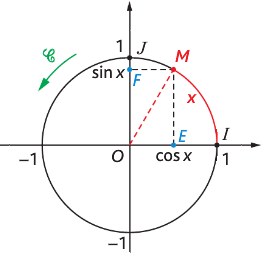
\includegraphics[width=0.35\textwidth]{images/14_cercl4.PNG}
\end{center}

\begin{exemples}
\begin{itemize}
    \item Le nombre réel $\dfrac{\pi}{2}$ correspond au point $J$, d'où $\cos\dfrac{\pi}{2}=0$ et $\sin\dfrac{\pi}{2}=1$.
    \item Le nombre réel $0$ correspond au point $I$, d'où $\cos(0)=1$ et $\sin(0)=0$.
    \item Pour $-\dfrac{\pi}{2}$, on a $\cos\left(-\dfrac{\pi}{2}\right)=0$ et $\sin\left(-\dfrac{\pi}{2}\right)=-1$.
\end{itemize}
\end{exemples}

\medskip
\noindent\textbf{Lien avec les formules de trigonométrie dans le triangle rectangle $OEM$.}

Si $x\in\left[0;\dfrac{\pi}{2}\right]$ (le raisonnement est analogue sur les autres intervalles, mais il faut faire attention aux signes) :
\[
\cos(\widehat{EOM})=\frac{\text{côté adjacent}}{\text{hypoténuse}}
=\frac{OE}{OM}=\frac{OE}{1}=\cos(x),
\]
\[
\sin(\widehat{EOM})=\frac{\text{côté opposé}}{\text{hypoténuse}}
=\frac{EM}{OM}=\frac{EM}{1}=\sin(x).
\]

\subsection{Propriétés}

\begin{propriete}
Pour tout réel $x$, on a :
\begin{itemize}
    \item $-1\leq \cos x\leq 1$ et $-1\leq \sin x\leq 1$ ;
    \item $\cos^2 x+\sin^2 x=1$.
\end{itemize}
\end{propriete}

\begin{remarque}
$\cos^2 x$ et $\sin^2 x$ s'écrivent aussi $(\cos x)^2$ et $(\sin x)^2$.
\end{remarque}

\begin{demonstration}
La première propriété découle directement de la définition, le cercle trigonométrique étant de rayon $1$.

La deuxième propriété se démontre avec le théorème de Pythagore, par disjonction de cas (étude de tous les cas possibles).

Pour $x\in\left]0;\dfrac{\pi}{2}\right[$, dans le triangle $OEM$ rectangle en $E$ :
\[
OE^2+EM^2=OM^2
\quad\Longleftrightarrow\quad
\cos^2 x+\sin^2 x=1.
\]
Le résultat est valable par symétrie sur les intervalles
$\left[\dfrac{\pi}{2};\pi\right[$,
$\left]-\pi;-\dfrac{\pi}{2}\right[$ et
$\left]-\dfrac{\pi}{2};0\right[$.

Les cas particuliers $0$, $\dfrac{\pi}{2}$, $\pi$ et $-\dfrac{\pi}{2}$ se vérifient par calcul.
\end{demonstration}

\subsection{Valeurs remarquables}

\begin{center}
\small
\renewcommand{\arraystretch}{1.5}
\begin{tabular}{|c|c|c|c|c|c|c|}
\hline
Valeur de $x$ en radians & $0$ & $\dfrac{\pi}{6}$ & $\dfrac{\pi}{4}$ & $\dfrac{\pi}{3}$ & $\dfrac{\pi}{2}$ & $\pi$ \\
\hline
$\sin x$ & $0$ & $\dfrac12$ & $\dfrac{\sqrt2}{2}$ & $\dfrac{\sqrt3}{2}$ & $1$ & $0$ \\
\hline
$\cos x$ & $1$ & $\dfrac{\sqrt3}{2}$ & $\dfrac{\sqrt2}{2}$ & $\dfrac12$ & $0$ & $-1$ \\
\hline
\end{tabular}
\end{center}

\begin{center}
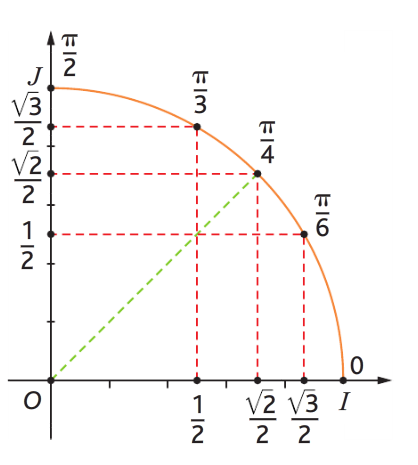
\includegraphics[width=0.4\textwidth]{images/14_angrem.PNG}
\end{center}

\begin{demonstration}
\begin{enumerate}[label=\arabic*.]
    \item Démontrons que $\sin\left(\dfrac{\pi}{4}\right)=\dfrac{\sqrt2}{2}$.

    La mesure $\dfrac{\pi}{4}$ rad est égale à la mesure $45^\circ$.
    \begin{center}
    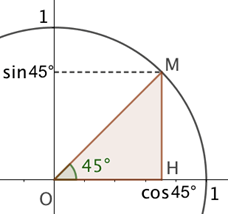
\includegraphics[width=0.17\textwidth]{images/trigonometrie_1.png}
    \end{center}
    Le triangle $OHM$ est rectangle et isocèle en $H$ ; en effet, l'angle $\widehat{OMH}$ est égal à $180^\circ-90^\circ-45^\circ=45^\circ$.

    Donc $HO=HM$, et donc $\sin\left(\dfrac{\pi}{4}\right)=\cos\left(\dfrac{\pi}{4}\right)$. Or,
    \begin{align*}
    \cos^2\left(\frac{\pi}{4}\right)+\sin^2\left(\frac{\pi}{4}\right)&=1\\
    2\sin^2\left(\frac{\pi}{4}\right)&=1\\
    \sin^2\left(\frac{\pi}{4}\right)&=\frac12\\
    \sin\left(\frac{\pi}{4}\right)&=\sqrt{\frac12}=\frac{1}{\sqrt2}=\frac{\sqrt2}{2},
    \end{align*}
    car $\sin\left(\dfrac{\pi}{4}\right)$ est positif.

    \item Démontrons que $\cos\left(\dfrac{\pi}{3}\right)=\dfrac12$ et $\sin\left(\dfrac{\pi}{3}\right)=\dfrac{\sqrt3}{2}$.

    La mesure $\dfrac{\pi}{3}$ rad est égale à la mesure $60^\circ$.
    \begin{center}
    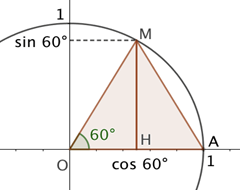
\includegraphics[width=0.20\textwidth]{images/trigonometrie_2.png}
    \end{center}
    Le triangle $OMA$ est isocèle en $O$ ; en effet, $OA=OM$. Les angles $\widehat{OMA}$ et $\widehat{MAO}$ sont égaux à $(180^\circ-60^\circ)/2=60^\circ$. Le triangle $OMA$ est donc équilatéral.

    Ainsi, la hauteur $(MH)$ est également une médiane du triangle. Elle coupe donc $[OA]$ en son milieu. On a donc $\cos\left(\dfrac{\pi}{3}\right)=\dfrac12$. Or,
    \begin{align*}
    \cos^2\left(\frac{\pi}{3}\right)+\sin^2\left(\frac{\pi}{3}\right)&=1\\
    \left(\frac12\right)^2+\sin^2\left(\frac{\pi}{3}\right)&=1\\
    \sin^2\left(\frac{\pi}{3}\right)&=1-\frac14=\frac34\\
    \sin\left(\frac{\pi}{3}\right)&=\sqrt{\frac34}=\frac{\sqrt3}{2},
    \end{align*}
    car $\sin\left(\dfrac{\pi}{3}\right)$ est positif.
\end{enumerate}
\end{demonstration}

\begin{remarque}
On en déduit le schéma suivant :
\begin{center}
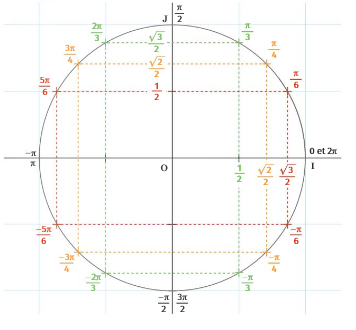
\includegraphics[width=0.42\textwidth]{images/cerc_cos_sin.png}
\end{center}
\end{remarque}

\section{Propriétés des fonctions cosinus et sinus}

\subsection{Définition}

\begin{definition}
\begin{itemize}
    \item La fonction qui, à tout réel $x$, associe le nombre $\cos(x)$ est appelée \emph{fonction cosinus}.
    \item La fonction qui, à tout réel $x$, associe le nombre $\sin(x)$ est appelée \emph{fonction sinus}.
\end{itemize}
Elles sont toutes deux définies sur $\RR$, à valeurs dans l'intervalle $[-1;1]$.
\end{definition}

\subsection{Périodicité}

\begin{propriete}
Les fonctions cosinus et sinus sont \emph{$2\pi$-périodiques}, c'est-à-dire que, pour tout nombre réel $x$ et pour tout entier relatif $k$ :
\[
\cos(x+2k\pi)=\cos(x)
\qquad\text{et}\qquad
\sin(x+2k\pi)=\sin(x).
\]
\end{propriete}

\begin{exemples}
\begin{itemize}
    \item $\cos(x+36\pi)=\cos(x+2\times18\pi)=\cos(x)$.
    \item $\sin(2\pi-x)=\sin(-x)$.
\end{itemize}
\end{exemples}

\subsection{Parité}

\begin{propriete}
\begin{itemize}
    \item La fonction cosinus est une \emph{fonction paire}, c'est-à-dire que, pour tout nombre réel $x$ :
    \[
    \cos(-x)=\cos(x).
    \]
    \item La fonction sinus est une \emph{fonction impaire}, c'est-à-dire que, pour tout nombre réel $x$ :
    \[
    \sin(-x)=-\sin(x).
    \]
\end{itemize}
\end{propriete}

\begin{remarque}
Cela repose encore sur la définition du cosinus et du sinus par enroulement de la droite réelle sur le cercle trigonométrique et les propriétés de symétrie.
\end{remarque}

\begin{exemples}
\begin{itemize}
    \item $\cos(-x+14\pi)=\cos(-x+2\times7\pi)=\cos(-x)=\cos(x)$.
    \item $\sin(22\pi-x)=\sin(2\times11\pi-x)=\sin(-x)=-\sin(x)$.
\end{itemize}
\end{exemples}

\section{Variations des fonctions cosinus et sinus}

\begin{propriete}
\textbf{(Admise)}
\begin{itemize}
    \item La fonction cosinus est décroissante sur $[0;\pi]$.
    \item La fonction sinus est croissante sur $[0;\pi/2]$ et décroissante sur $[\pi/2;\pi]$.
\end{itemize}
\end{propriete}

En utilisant la parité des fonctions cosinus et sinus, on obtient leurs tableaux de variations sur l'intervalle $[-\pi;\pi]$ :

\begin{center}
\renewcommand{\arraystretch}{1.4}
\begin{tabular}{c|ccccc}
$x$ & $-\pi$ & & $0$ & & $\pi$ \\
\hline
Variations de $\cos$ & $-1$ & $\nearrow$ & $1$ & $\searrow$ & $-1$ \\
Variations de $\sin$ & $0$ & $\searrow$ & $0$ & $\nearrow$ & $0$
\end{tabular}
\end{center}

Pour faire apparaître les extrema intermédiaires, les points remarquables sont $-\pi$, $-\pi/2$, $0$, $\pi/2$ et $\pi$. Ainsi, $\sin(-\pi/2)=-1$, $\sin(\pi/2)=1$, et $\cos(-\pi/2)=\cos(\pi/2)=0$.

Les variations des fonctions cosinus et sinus sur $\RR$ se déduisent de leurs variations sur l'intervalle $[-\pi;\pi]$ en utilisant la $2\pi$-périodicité de ces deux fonctions.

\section{Représentations graphiques des fonctions cosinus et sinus}

\begin{definition}
Dans le plan muni d'un repère orthogonal $(O,\vec{i},\vec{j})$, les fonctions cosinus et sinus sont représentées par deux courbes appelées \emph{sinusoïdes}.
\end{definition}

\begin{center}
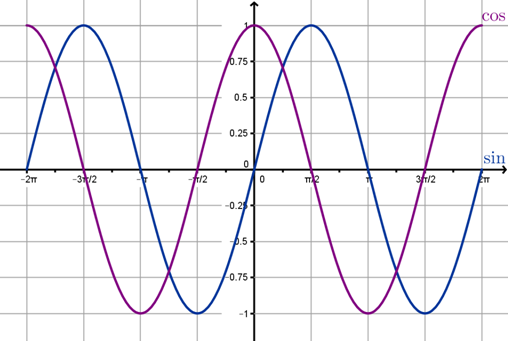
\includegraphics[width=0.5\textwidth]{images/Representations_graphiques_sinus_cosinus.png}
\end{center}

\begin{remarque}
\begin{itemize}
    \item Les courbes sont invariables par translation de vecteur $2\pi\vec{i}$ (périodicité).
    \item La courbe de la fonction cosinus est symétrique par rapport à l'axe des ordonnées (parité).
    \item La courbe de la fonction sinus est symétrique par rapport à $O$ (imparité).
\end{itemize}
\end{remarque}

\end{document}
